%!TEX root = report.tex
\chapter{Technical Details}
\par This chapter discusses the tools we used for process control, scheduled task management, and general project management.

\section{Process Control System - Supervisor}
\par We needed to monitor two daemon tasks. The first task was the script to send requests to TfL Live Bus Arrivals API and save the arrivals to the Databases (Section~\ref{sec:arrivals_daemon}). The second task was to keep Gunicorn running (Section~\ref{sec:gunicorn}).

\par We used Supervisor~\cite{supervisor} to monitor these two tasks. It watches the two processes and restart them if they fail, and ensure they start on system boot.

\par Supervisor was chosen as it matches our requirement exactly, as it is meant to be used to control processes related to a project or a customer, and is meant to start like any other program at boot time.

\section{Scheduled Tasks Management - Jenkins}
\par We used Jenkins \cite{jenkins} to managed our predictions timetable update schedule. Figure \ref{fig:jenkins} shows some of our schedule tasks. Jenkins was chosen as it provides a dashboard that gives a quick glance of the build state and saves build histories for future reference.

\begin{figure}
\centering
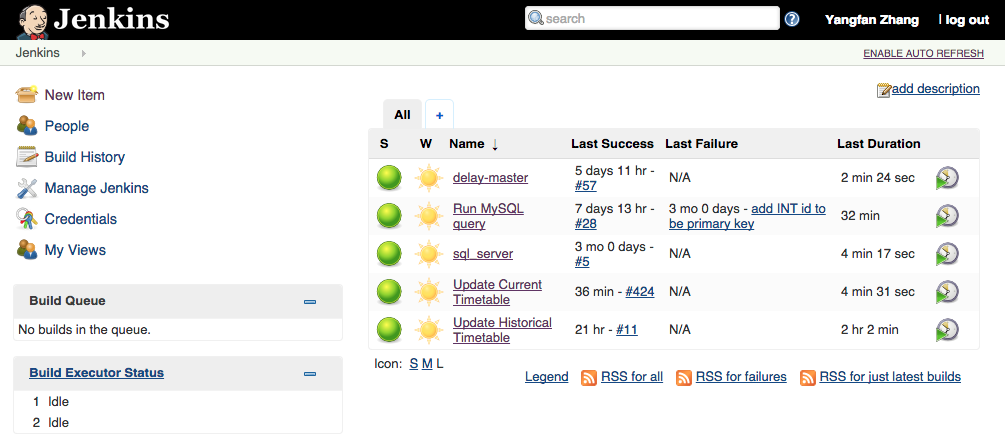
\includegraphics[width=\textwidth]{figures/jenkins.png}
\caption{\label{fig:jenkins} Jenkins Dashboard}
\end{figure}

\subsection{Current Timetable Update}
\par The current timetable is re-generated every hour. We set up a Jenkins job to re-run the relevant current timetable update SQL script every hour, and save the previous timetable into a log for updating the historical timetable at a later time. This job takes less than 10 minutes on average.

\subsection{Historical Timetable Update}
\par Similarly, we set up a Jenkins job to update the Historical Timetable daily at 3.30am when the server is less busy.

\subsection{Arrivals Daily Backup}
\par The arrivals table grows rapidly with an additional 150,000 rows every hour. In order to allow fast access to the arrivals within the past one hour to construct the current timetable, we decided to save the arrivals for the current day in a new table, while keeping the past arrivals entries in an archive table. This required us to backup the arrivals entries daily to the archive.

\par Again, we created a Jenkins job to run the back up script daily. In order not to affect the historical timetable update, we set this job as a downstream task of the historical timetable update.

\section{Software Project Management -- Trello}
\par We used Trello \cite{trello} for project management. It was useful to keep track of the tasks backlog, the tasks at hand, and the tasks to be further tested (Figure \ref{fig:trello}). We chose Trello because it is free, and has a simple user interface.

\begin{figure}
\centering
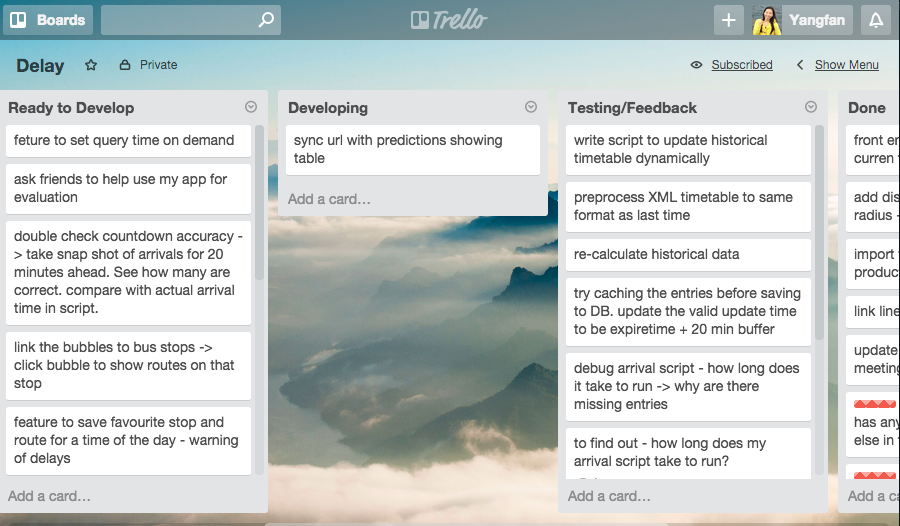
\includegraphics[width=\textwidth]{figures/trello_small.png}
\caption{\label{fig:trello} Project Trello Board}
\end{figure}

\section{Summary}
\par The appropriate use of the above tools makes it easy to keep track of daemon processes and regularly scheduled tasks, and manage the pace of development. This makes development and deployment much smoother.
